\documentclass[12pt]{scrartcl}

\usepackage[utf8]{inputenc}
\usepackage[T1]{fontenc}
\usepackage{lmodern}
\usepackage{graphicx}
\usepackage[pdftex,hyperref,dvipsnames]{xcolor}
\usepackage{listings}
\usepackage[a4paper,lmargin={2cm},rmargin={2cm},tmargin={3.5cm},bmargin = {2.5cm},headheight = {4cm}]{geometry}
\usepackage{amsmath,amssymb,amstext,amsthm}
% \usepackage[lined,algonl,boxed]{algorithm2e} 
\usepackage{algpseudocode}
\usepackage{tikz}
\usepackage{pgfplots}
\usepackage{hyperref}
\usepackage{url}
\usepackage{tcolorbox}
\usepackage{float}
\usepackage[inline]{enumitem}
\usepackage[headsepline]{scrlayer-scrpage} 

\usetikzlibrary{automata,positioning}

\usepgfplotslibrary{external}
%\tikzexternalize
\pgfplotsset{width=10cm,compat=1.9}
\pgfplotsset{every axis/.style={
    axis line style = thick,
    grid = both,
    tick pos = left,
    tick align = outside,
    tick style = {thick,black},
    fill = blue,
	line width = 2pt,
}}

\lstset{
  basicstyle=\ttfamily\small,
  numbers=left,
  numberstyle=\tiny,
  stepnumber=1,
  numbersep=8pt,
  frame=single,
  breaklines=true,
  columns=fullflexible
}

\lstset{
  language=C,
  basicstyle=\ttfamily\small,
  keywordstyle=\color{blue},
  commentstyle=\color{gray},
  stringstyle=\color{green!60!black},
  numbers=left,
  numberstyle=\tiny,
  stepnumber=1,
  numbersep=8pt,
  frame=single,
  breaklines=true,
  columns=fullflexible
}

\renewcommand{\theenumi}{(\alph{enumi})}
\renewcommand{\labelenumi}{\text{\theenumi}}
\renewcommand{\labelenumii}{(\roman{enumii})} 

\ohead{Weiting Wang (3855168)\\
       Nico Strohbach (3546914)\\
       Jan Theil (3794698)}

\ihead{Reinforcement Learning}

\newcounter{exnum}
\newcommand{\exercise}[1]{\section*{Problem \theexnum\stepcounter{exnum}: #1}}

\begin{document}

\setcounter{exnum}{1}
\exercise{Linear function approximation}

\begin{enumerate}
  \item Instead of holding all the values of the value function $v(s_i) = w_i$ as a table, one could simulate this by using linear function approximation with unit vectors.
        The feature vector for a state $s_i$ would look like this: $x(s_i) = \left[ x_1(s_i), x_2(s_i), \ldots, x_d(s_i) \right]^T$ with $d = |S|$ and $x_i(s_i) = 1, \forall_{j \neq i} x_j(s_i) = 0$.
        This is basically $x(s_i) = e_i$ ($e_i$ being the unit vector with $1$ at position $i$). Thus, the value function would be $\hat{v}(s_i, w) = w^T x(s_i) = w^T e_i = w_i$, which
        is the same as the (tabular) value function definition above. 
  \item \begin{itemize}
    \item Tabular case: $Q(S_t, A_t) \leftarrow Q(S_t, A_t) + \alpha \left[ R_{t+1} + \gamma Q(S_{t+1}, A_{t+1}) - Q(S_t, A_t) \right]$
    \item Function approximation (general case): Using action-value function approximation $\hat{q}(s, a, w)$ and $U_t = R_{t+1} + \gamma \hat{q}(S_{t+1}, A_{t+1}, w)$:
          $\\w_{t+1} = w_t + \alpha \left[ R_{t+1} + \gamma \hat{q}(S_{t+1}, A_{t+1}, w) - \hat{q}(S_t, A_t, w_t) \right] \nabla \hat{q}(S_t, A_t, w_t)$
    \item Linear function approximation: Using $\hat{q}(s, a, w) = w^T x(s, a) = \sum_{i = 1}^d w_i x_i(s, a)$ and $\nabla \hat{q}(s, a, w) = x(s, a)$:
          $\\w_{t+1} = w_t + \alpha \left[ R_{t+1} + \gamma  w_t^T x(S_{t+1}, A_{t+1}) - w_t^T x(S_t, A_t) \right] x(s, a)$
  \end{itemize}
\end{enumerate}

\exercise{Mountain Car}

\begin{enumerate}
  \item For the source code please see \textit{ex07-fa.py}. \begin{figure}[H]
    \centering
    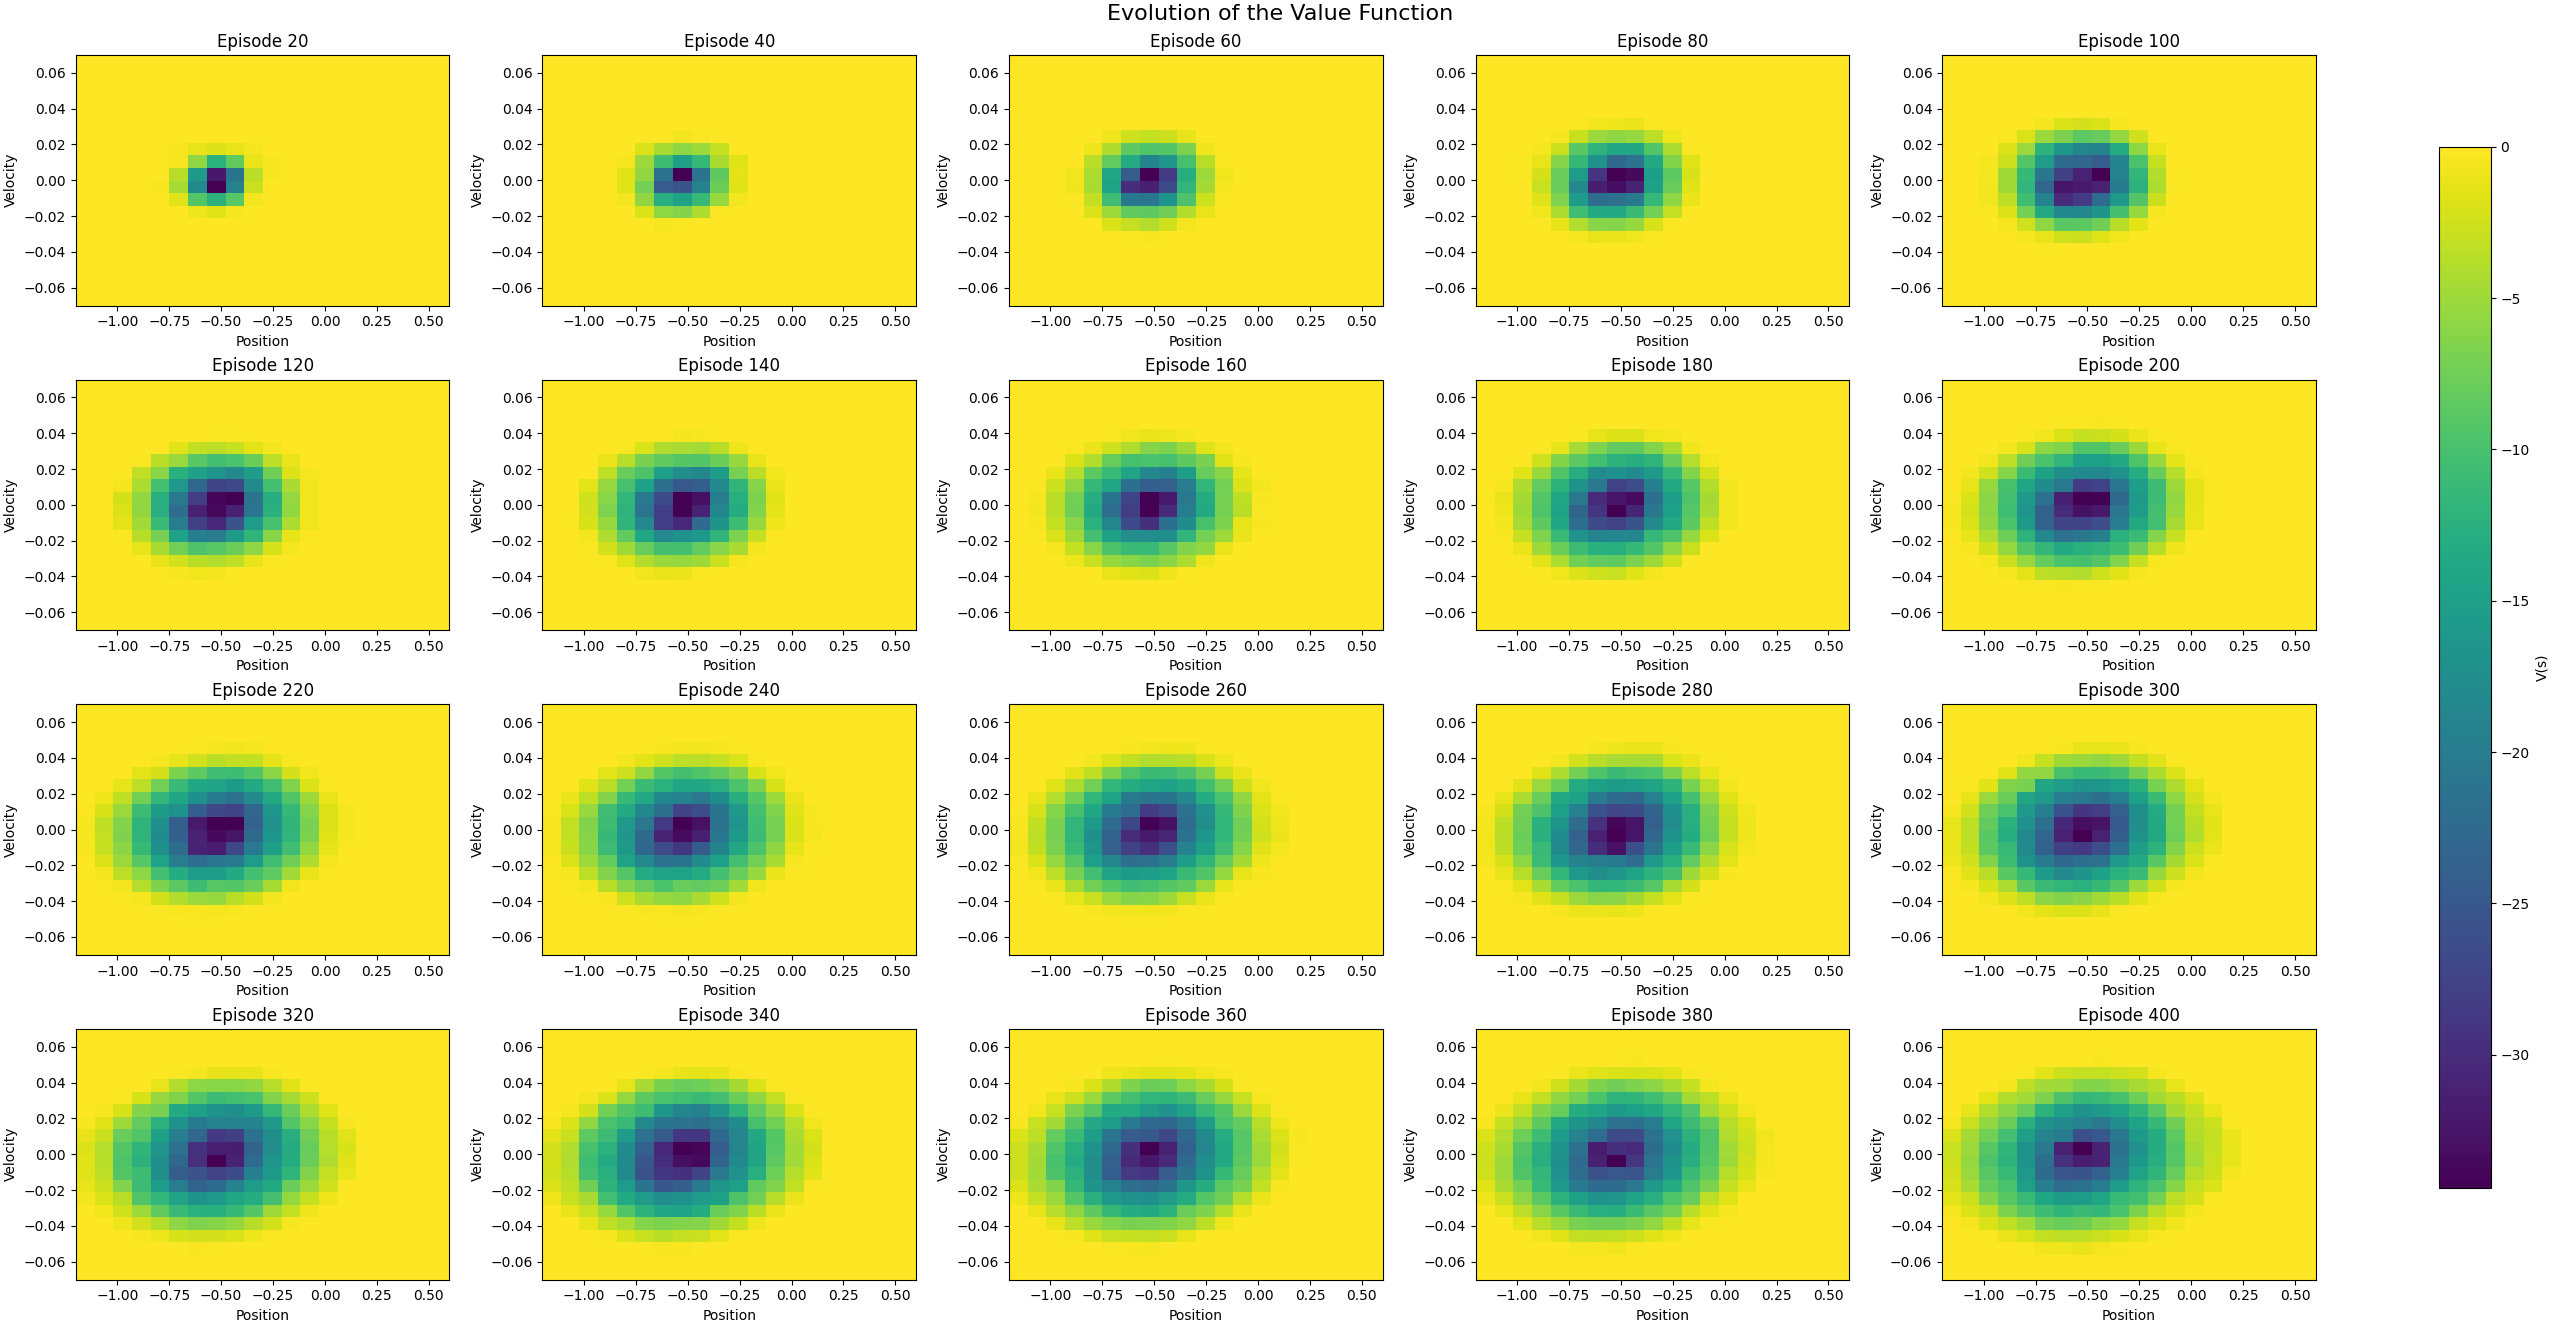
\includegraphics[width=\textwidth]{1.png}
    \caption{Value function every 20 episodes}
    \label{fig:1}
  \end{figure}
  \item For the source code please see \textit{ex07-fa-b.py}. \begin{figure}[H]
    \centering
    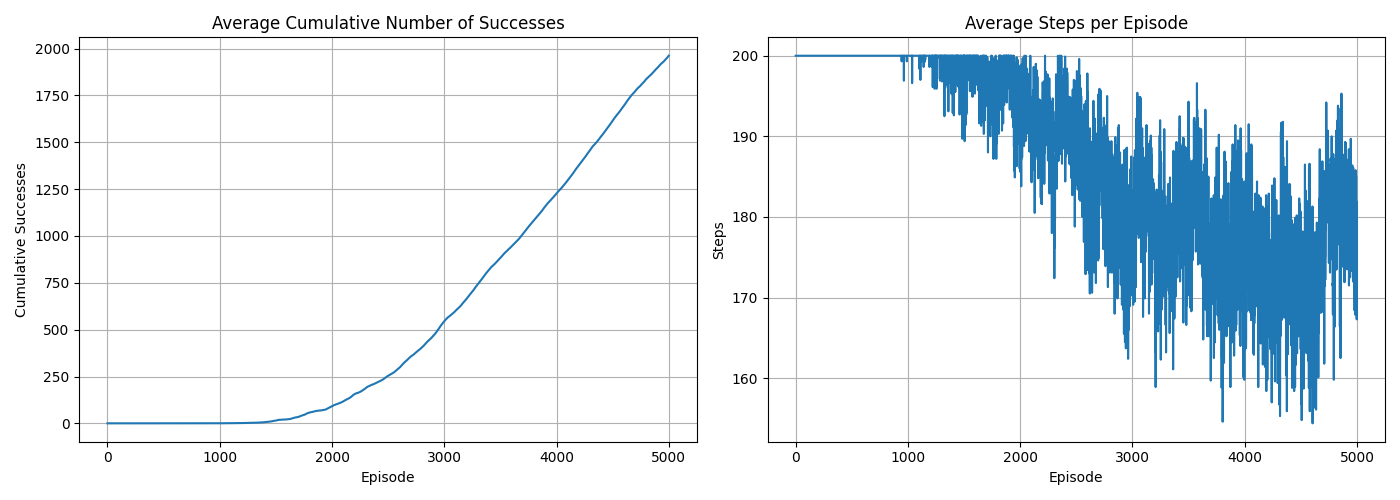
\includegraphics[width=\textwidth]{2.png}
    \label{fig:2}
  \end{figure}
  It seems to take around 1500 episodes on average to discover a strategy of reaching the top. 
  Once a this pendulum strategy is discovered the number of steps per episode decreases during optimization of
  said strategy.
  \item 
\end{enumerate}

\end{document}